\chapter{Discussion} \label{discussion}
In Figure \ref{data_newk} the difference in output from running the model with the new $\kappa$-values, Euro code $\kappa$ and the measured data can be seen. 
The improved accuracy is clear from in Table \ref{errortab} as the error for the model using MCMC values is consistently smaller than the error incurred by the same model using the Euro-code thermal conductivity ($\kappa$) values.
There are instances where the error from the model using the MAP $\kappa$-values is smaller than the model using the MCMC $\kappa$-values. 
This should not discredit the usage and value of the Markov Chain Monte-Carlo algorithm as the increased accuracy from the MAP values is only marginal.
It is also important to remember that the MAP optimization did not truly find the maximum at every point and that due to insufficient iterations the results from the MAP optimization was at some temperatures closer to the results from the MCMC algorithm than to the true maximum.

\begin{figure}
	\label{data_newk}
	\centering
	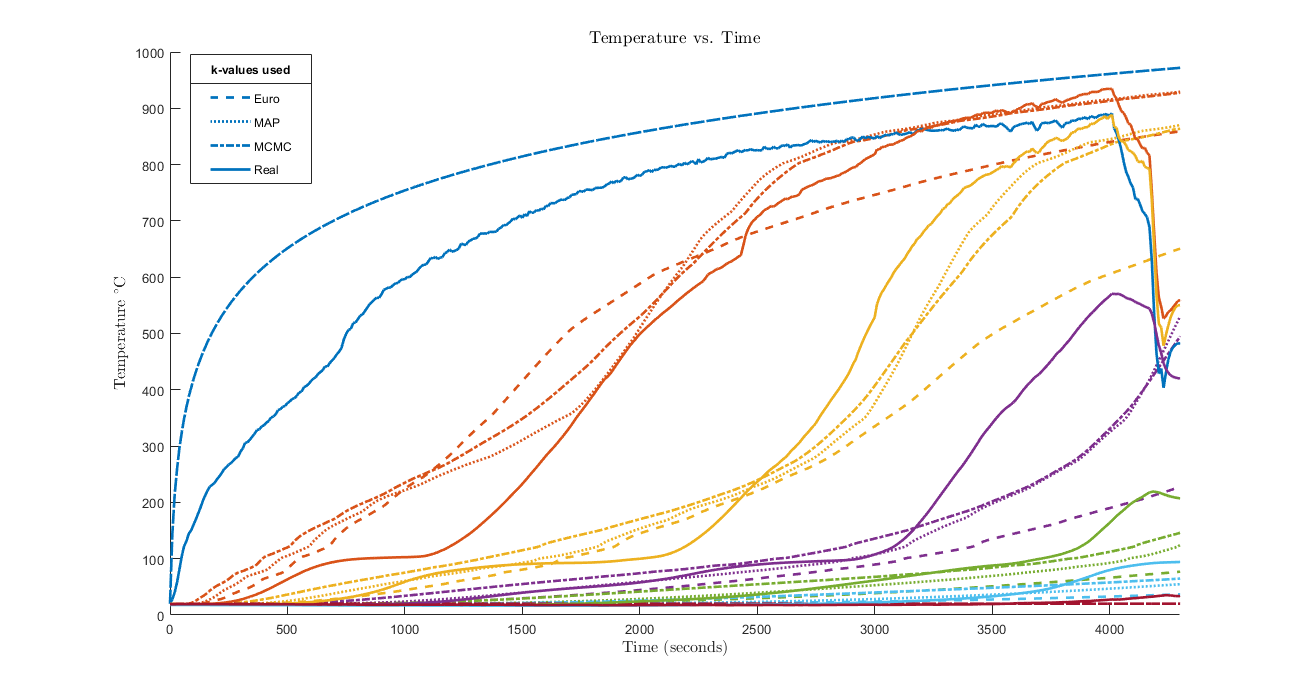
\includegraphics[width=\textwidth,]{figures/final_graph.png}
\end{figure}
%    Summarize the important findings of your observations.
The $\kappa$-values obtained from the MAP and MCMC analysis give a more accurate model output than those from the Euro-code.
The increased accuracy that the new $\kappa$-values provide, serves as a proof of concept that MCMC analysis can be used to determine more accurate fire ratings and specifically fire resistance. 

Fire resistance is measured in minutes, this indicates the amount of time from the start of the fire until a specific condition is met. 
The main conditions taken into account are accounted for by the REI marker system \citep{rei:2021}. 
Where `R' indicates the load-bearing capacity of the structural element, the associated time indicates when the element can no longer carry the design load.
`E' refers to the integrity of the element and the time indicates how long after ignition the fire penetrates the element a `I', indicates insulation ability, a limit is set to the temperature of the non-heated side.
Time corresponding with that rating refers to when that temperature is exceeded on the non-heated side.

With further development of analytical determination of thermal conductivity and applied finite element models, the data obtained from fire test could be used in a model to determine the REI markers of different size elements.
%    For each result, describe the patterns, principles, relationships your results show. Explain how your results relate to expectations and to references cited. Explain any agreements, contradictions, or exceptions. Describe what additional research might resolve contradictions or explain exceptions.

%    Suggest the theoretical implications of your results. Extend your findings to other situations or other species. Give the big picture: do your findings help us understand a broader topic?
The accuracy of the Markov Chain Monte-Carlo analysis can be increased by modelling the standard deviation, of both the temperatures and the $\kappa$ values, as random values and solving for them as well. 
This would make the analysis more heuristic and decrease the dependence of the results on assumptions made by the researcher. 
Additionally the program could've been run for a longer time to ensure more samples. and thereby a more accurate approximation of the population mean. 
Unfortunately the main limitation in this project was computational time.

The MAP analysis could be fine-tuned yet that would be pointless as it is already known that the probability of the thermal conductivity is not symmetrically distributed and that the mean is a more accurate description of the data than the Maximum a posteriori.


In retrospect there should have been more cleaning of the measured data before analysis was done. Inaccuracies arose due to the first 90 sec of the measurements being taken before the furnace was turned on and the thermocouples still measuring after the fire died down.
These measurement discrepancies between model and measurement should have been better taken into account and excluded form modelling. 

This research can be expanded and applied to the measured data available for Eucalyptus. 
Applying the same algorithm to different data sets and obtaining accurate modelling from both data sets would be confirmation that the algorithm is accurate enough to be further explored for usage in practice.



